% Unit 124 terjemahan Bahasa Indonesia dari chapter9.tex baris 818--950.
% Sumber: Methods of Algebra, Volume 2, commit
% 9a5803ff77dd3257484cb177f851a73770a59dd3 (CC BY 4.0).
% stable-unit-id: o014.aljabr2.chapter9.duality-examples-a
% Cakupan: Bagian 9.3 dari ruang vektor hingga contoh kobordisme.

% segment-id: o014.li2.chapter9.duality-examples-a.h001
\section{Contoh-contoh dualitas}\label{sec:duality-examples}
\hypertarget{o014.aljabr2.chapter9.duality-examples-a}{ }
% segment-id: o014.li2.chapter9.duality-examples-a.p001
Selanjutnya kita telaah beberapa contoh dasar teori dualitas.

% segment-id: o014.li2.chapter9.duality-examples-a.eg001
\begin{example}\label{eg:Vect-trace}
	Tinjau kategori ruang vektor di atas medan $\Bbbk$,
	$\cate{Vect}(\Bbbk)$, dengan struktur monoidal simetris standarnya dan
	unit $\munit:=\Bbbk$. Inilah model utama dualitas.
	Proposisi~\ref{prop:dualizable-module} menyiratkan bahwa, untuk setiap ruang
	vektor-$\Bbbk$ $V$,
	% segment-id: o014.li2.chapter9.duality-examples-a.q001
	\[ V \;\text{memiliki dual} \iff V \;\text{berdimensi hingga}. \]
	Lebih konkret, untuk ruang vektor-$\Bbbk$ berdimensi $n$, dualnya
	(tanpa perlu membedakan kiri dan kanan) diambil sebagai
	% segment-id: o014.li2.chapter9.duality-examples-a.q002
	\[ V^* := \Hom_{\Bbbk}(V, \Bbbk), \]
	dengan morfisme-morfisme yang bersesuaian
	% segment-id: o014.li2.chapter9.duality-examples-a.q003
	\[\begin{tikzcd}[row sep=tiny]
		V \otimes V^* \arrow[r, "{\mathrm{ev}}"] & \Bbbk \\
		v \otimes \check{v} \arrow[mapsto, r] & \check{v}(v)
	\end{tikzcd} \quad \begin{tikzcd}[row sep=tiny]
		\Bbbk \arrow[r, "{\mathrm{coev}}"] & V^* \otimes V \\
		1 \arrow[mapsto, r] & \sum_{i=1}^n \check{v}_i \otimes v_i.
	\end{tikzcd} \]
	Di sini $v_1,\ldots,v_n$ adalah sembarang basis dari $V$, sedangkan
	$\check v_1,\ldots,\check v_n$ basis dualnya. Definisi-definisi ini
	merupakan kasus khusus Proposisi~\ref{prop:dualizable-module}, dan dapat
	pula diperiksa langsung tanpa kesulitan.

	\index[sym1]{Vectf@$\cate{Vect}_{\mathrm{f}}$}
	Ruang vektor-$\Bbbk$ berdimensi hingga membentuk kategori kaku terhadap
	$\otimes$, yang dinotasikan oleh $\cate{Vect}_{\mathrm f}(\Bbbk)$.
	Semua operasi yang melibatkan dual menjadi fakta-fakta elementer berikut.
	\begin{itemize}
		\item Isomorfisme
		$V^*\otimes W\simeq\Hom(\Bbbk,V^*\otimes W)\rightiso\Hom(V,W)$
		memetakan $\sum_i\check v_i\otimes w_i$ ke pemetaan linear
		$\sum_i\check v_i(\mathord\cdot)w_i$.
		\item Dual $f^*:W^*\to V^*$ dari morfisme $f:V\to W$ tepat merupakan
		transpos pemetaan linear; persamaan diagramatik
		\eqref{eqn:f-dual-ev} mencakup seluruh isinya.
		\item Jejak dan dimensi mengambil nilai dalam
		$\End(\Bbbk)\simeq\Bbbk$. Karena
		$\cate{Vect}_{\mathrm f}(\Bbbk)$ simetris, tidak perlu membedakan
		versi kiri dan kanan.
		\item Setelah $\End(V)$ diidentifikasikan dengan $V^*\otimes V$,
		% segment-id: o014.li2.chapter9.duality-examples-a.q004
		\[ \Tr\left(\sum_i\check v_i\otimes v_i\right)=
		\sum_i\check v_i(v_i) \]
		tepat merupakan jejak klasik. Demikian pula, $\dim V$ ialah bayangan
		dimensi klasik di bawah homomorfisme $\Z\to\Bbbk$.
	\end{itemize}
\end{example}

% segment-id: o014.li2.chapter9.duality-examples-a.eg002
\begin{example}\label{eg:superVect-trace}
	\index{ruang vektor super@ruang vektor super}
	Tinjau kategori monoidal simetris
	$\cate{Vect}^-_{\Z/2\Z}(\Bbbk)$ dari Contoh~\ref{eg:superspace}.
	Objek dan morfismenya masing-masing ditulis sebagai
	$V=V_0\oplus V_1$ dan $f=(f_0,f_1)$, dengan
	$\Bbbk=\Bbbk\oplus\{0\}$ sebagai unit. Seperti dalam
	Contoh~\ref{eg:Vect-trace}, sebuah objek $V$ memiliki dual jika dan
	hanya jika ia berdimensi hingga sebagai ruang vektor-$\Bbbk$; semua
	objek ini membentuk subkategori penuh
	$\cate{Vect}^-_{\Z/2\Z, f}(\Bbbk)$. Jika $V$ berdimensi hingga, dualnya
	dapat diambil sebagai
	% segment-id: o014.li2.chapter9.duality-examples-a.q005
	\[ V^* = V^*_0 \oplus V^*_1, \quad V^*_i := \Hom_{\Bbbk}(V_i, \Bbbk), \]
	dengan
	% segment-id: o014.li2.chapter9.duality-examples-a.q006
	\[\begin{tikzcd}[row sep=tiny, column sep=small]
		V \otimes V^* \arrow[r, "{\mathrm{ev}}"] & \Bbbk \\
		(v_0, v_1) \otimes (\check{v}_0, \check{v}_1) \arrow[mapsto, r] & \check{v}_0(v_0) - \check{v}_1(v_1), \\
		\Bbbk \arrow[r, "{\mathrm{coev}}"] & V^* \otimes V \\
		1 \arrow[mapsto, r] & \sum_{i=1}^{n_0} \check{v}_{0,i} \otimes v_{0,i} - \sum_{i=1}^{n_1} \check{v}_{1,i} \otimes v_{1,i}.
	\end{tikzcd}\]
	Di sini $v_{0,1},\ldots,v_{0,n_0}$ (atau
	$v_{1,1},\ldots,v_{1,n_1}$) adalah sembarang basis dari $V_0$ (atau
	$V_1$), sedangkan $\check v_{0,1},\ldots,\check v_{0,n_0}$ (atau
	$\check v_{1,1},\ldots,\check v_{1,n_1}$) basis dualnya. Syarat-syarat
	dalam Definisi~\ref{def:dualizable-obj} dapat diperiksa langsung.
	\begin{itemize}
		\item Isomorfisme
		$(V^*\otimes W)_0\simeq\Hom(\Bbbk,V^*\otimes W)
		\rightiso\Hom(V,W)$ memetakan $\sum_i\check v_i\otimes w_i$ ke
		pemetaan linear $\sum_i\check v_i(\mathord\cdot)w_i$, dengan
		$\check v_i\in V_0^*$ dan $w_i\in W_0$, atau
		$\check v_i\in V_1^*$ dan $w_i\in W_1$.
		\item Dual $f^*:W^*\to V^*$ dari morfisme $f:V\to W$ tetap
		transpos pemetaan linear, diterapkan secara terpisah pada setiap suku
		jumlah langsung.
		\item Jejak dan dimensi tetap mengambil nilai dalam
		$\End(\Bbbk)\simeq\Bbbk$, tanpa membedakan kiri dan kanan. Jejak
		endomorfisme $f=(f_0,f_1)\in\End(V)$ ialah
		$\Tr(f_0)-\Tr(f_1)$ dan disebut \emph{superjejak}. Sejalan dengan itu,
		\emph{superdimensi} $\dim V$ ialah bayangan
		$\dim V_0-\dim V_1$ di bawah $\Z\to\Bbbk$.
	\end{itemize}

	Deskripsi serupa berlaku bagi kategori ruang vektor-$\Bbbk$ bergradasi
	yang lebih umum, $\cate{Vect}^{\epsilon}_I(\Bbbk)$, dengan $I$ monoid
	komutatif dan $\epsilon:I\to\Z/2\Z$; lihat
	Contoh~\ref{eg:graded-module}. Objek dan morfisme kategori monoidal
	simetris ini tetap berbentuk $\bigoplus_{i\in I}V_i$ dan
	$(f_i)_{i\in I}$, sedangkan tanda-tandanya bergantung pada $\epsilon(i)$.
\end{example}

% segment-id: o014.li2.chapter9.duality-examples-a.p002
Perhatikan bahwa $\cate{Vect}(\Bbbk)$ membenam ke
$\cate{Vect}^-_{\Z/2\Z}(\Bbbk)$ melalui
$V\mapsto(V_0,V_1):=(V,\{0\})$. Karena itu,
Contoh~\ref{eg:superVect-trace} mencakup teori klasik dalam
Contoh~\ref{eg:Vect-trace}. Lebih jauh, jika $\Bbbk\in\{\R,\CC\}$,
ruang vektor super-$\Bbbk$ dapat diperumum menjadi berkas vektor super di
atas manifold topologis $M$. Superjejak dan superdimensi juga meluas ke
berkas vektor super; satu-satunya perbedaan ialah bahwa nilainya berada
dalam monoid endomorfisme berkas vektor super trivial
$M\times(\Bbbk\oplus\{0\})$, yakni dalam
$\{\text{fungsi kontinu }M\to\Bbbk\}$.

% segment-id: o014.li2.chapter9.duality-examples-a.p003
Berikutnya adalah dua contoh nonlinier.

% segment-id: o014.li2.chapter9.duality-examples-a.eg003
\begin{example}[Korespondensi]
	Misalkan $\mathrm{Corr}$ kategori berikut. Objeknya semua himpunan kecil,
	dan morfisme dari $X$ ke $Y$ didefinisikan sebagai kelas isomorfisme
	diagram $[X\xleftarrow{u}A\xrightarrow{v}Y]$, dengan $A$ sembarang himpunan kecil
	dan $u,v$ sembarang pemetaan; isomorfisme dipahami dengan cara
	yang jelas. Diagram semacam itu disebut ``korespondensi'' dari $X$ ke
	$Y$ dan memperumum pemetaan.\footnote{Jika $f:X\to Y$ pemetaan, ambil
	$A$ sebagai graf $f$.} Komposisi
	$[Y\leftarrow B\rightarrow Z]$ dengan
	$[X\leftarrow A\rightarrow Y]$ didefinisikan melalui hasil kali serat:
	% segment-id: o014.li2.chapter9.duality-examples-a.q007
	\[\begin{tikzcd}[row sep=small]
		& & A \dtimes{Y} B \arrow[ld] \arrow[rd] & & \\
		& A \arrow[ld] \arrow[rd] & & B \arrow[ld] \arrow[rd] & \\
		X & & Y & & Z.
	\end{tikzcd}\]
	Morfisme identitas objek $X$ ialah
	$X\xleftarrow{\identity}X\xrightarrow{\identity}X$, atau diagram
	sembarang yang isomorfik dengannya. Kasus-kasus khusus komposisi adalah
	% segment-id: o014.li2.chapter9.duality-examples-a.q008
	\begin{gather*}
		[Y = Y \xrightarrow{w} Z] \circ [X \xleftarrow{u} A \xrightarrow{v} Y] = [X \xleftarrow{u} A \xrightarrow{wv} Z ], \\
		[Y \xleftarrow{z} B \xrightarrow{w} Z] \circ [X \xleftarrow{u} Y = Y] = [X \xleftarrow{uz} B \xrightarrow{w} Z].
	\end{gather*}
	Himpunan abstrak digunakan di sini semata-mata untuk kepentingan
	pedagogis. Dalam penerapan, $X$, $Y$, dan seterusnya biasanya diambil
	sebagai objek geometris yang sesuai, seperti ruang topologis atau skema.

	Sekarang bekali $\mathrm{Corr}$ dengan struktur monoidal: definisikan
	$X\otimes Y:=X\times Y$, dengan himpunan satu titik $\mathrm{pt}$
	sebagai unit $\munit$. Kategori ini secara alami monoidal simetris dan
	juga kaku: untuk setiap $X$, ambil $X^*=X$ bersama
	% segment-id: o014.li2.chapter9.duality-examples-a.q009
	\[ \mathrm{coev}_X := \left[\begin{tikzcd}[row sep=tiny]
		\mathrm{pt} & X \arrow[l] \arrow[r, "\text{diagonal}"] & X \times X
	\end{tikzcd}\right], \quad
	\mathrm{ev}_X := \left[\begin{tikzcd}[row sep=tiny]
		X \times X & X \arrow[r] \arrow[l, "\text{diagonal}"'] & \mathrm{pt}.
	\end{tikzcd}\right] \]
	Pembaca dapat memeriksa dengan teliti syarat-syarat
	Definisi~\ref{def:dualizable-obj}.

	\begin{itemize}
		\item Setelah definisi dibentangkan, isomorfisme
		$\Hom_{\mathrm{Corr}}(X,Y)\simeq
		\Hom_{\mathrm{Corr}}(\munit,X^*\otimes Y)$ menjadi tautologi.
		\item Dual dari morfisme
		$f=[X\xleftarrow{u}A\xrightarrow{v}Y]$ ialah
		$f^*=[Y\xleftarrow{v}A\xrightarrow{u}X]$. Ini langsung terlihat
		dengan menjalankan definisi; perinciannya diserahkan kepada pembaca.
		\item Jejak dan dimensi mengambil nilai dalam
		$\End_{\mathrm{Corr}}(\munit)$. Unsur-unsur himpunan ini merupakan
		kelas isomorfisme diagram
		$[\mathrm{pt}\leftarrow A\rightarrow\mathrm{pt}]$ dan sepenuhnya
		ditentukan oleh kardinalitas $|A|$.
		\item Untuk sembarang pemetaan $u:A\to X$, tuliskan
		$\Gamma_u:=\{(a,u(a)):a\in A\}\subset A\times X$ untuk grafnya.
		Jejak endomorfisme
		$f=[X\xleftarrow{u}A\xrightarrow{v}X]$ dijelaskan oleh diagram
		% segment-id: o014.li2.chapter9.duality-examples-a.q010
		\[\begin{tikzcd}[row sep=small]
			& & &  \Gamma_u \cap \Gamma_v \arrow[hookrightarrow, ld] \arrow[hookrightarrow, rd] & & & \\
			& & \Gamma_u \arrow[ld, "\text{proyeksi}"'] \arrow[hookrightarrow, rd] & & \Gamma_v \arrow[hookrightarrow, ld] \arrow[rd, "\text{proyeksi}"] & & \\
			& X \arrow[ld] \arrow[rd, "\text{diagonal}"'] & & A \times X \arrow[ld, "{u \times \identity}"] \arrow[rd, "{v \times \identity}"'] & & X \arrow[ld, "\text{diagonal}"] \arrow[rd] & \\
			\mathrm{pt} & & X \times X & & X \times X & & \mathrm{pt}.
		\end{tikzcd}\]
		Setiap belah ketupat adalah persegi tarikan balik. Perhatikan bahwa
		$\Gamma_u\cap\Gamma_v\simeq\{a\in A:u(a)=v(a)\}$.

		Tuliskan $\Delta:=\Gamma_{\identity_X}\subset X\times X$ untuk
		subhimpunan diagonal. Dalam kasus khusus $A=X$ dan
		$u=\identity_X$, puncak diagram ialah himpunan titik tetap
		$\Gamma_v\cap\Delta=\{x\in X:v(x)=x\}$. Jadi fungsi $\Tr(f)$
		tepat menghitung titik tetap.

		\item Untuk kasus khusus $u=v=\identity_X$, tampak bahwa $\dim X$
		ialah perpotongan-diri diagonal $\Delta\cap\Delta$. Dalam situasi
		himpunan saat ini, $\Delta\cap\Delta$ sama dengan $X$, sehingga
		$\dim X\in\End_{\mathrm{Corr}}(\munit)$ hanya mendeskripsikan
		$|X|$. Dalam konteks geometri atau topologi yang lebih halus,
		bersama kerangka ``turunan'' yang sesuai, perpotongan-diri diagonal
		dapat memberikan informasi yang lebih halus dan penting.
	\end{itemize}
\end{example}

% segment-id: o014.li2.chapter9.duality-examples-a.eg004
\begin{example}[Kobordisme]
	\index{kobordisme@kobordisme (cobordism)}
	Tinjau kategori monoidal $n\dcate{Cob}$ dari
	\cite[Contoh 3.1.4]{Li1}. Objeknya manifold berorientasi kompak tanpa
	batas berdimensi $n-1$, dengan $n\in\Z_{\geq1}$, sedangkan morfismenya
	ialah kelas ekuivalensi ``kobordisme'' yang diwakili oleh manifold
	berorientasi berdimensi $n$ dengan batas; ekuivalensinya adalah
	difeomorfisme yang mempertahankan batas. Struktur monoidal berasal dari
	gabungan terpisah manifold berorientasi, dengan manifold kosong
	$\emptyset$ sebagai unit. Gambar konkret kobordisme, yang lazim disebut
	``celana'', dapat dilihat dalam rujukan tersebut. Namun agar sesuai
	dengan metode diagram dawai dalam \S\ref{sec:monoidal-dual}, kobordisme
	harus digambar dari atas ke bawah, bukan dari kiri ke kanan seperti dalam
	rujukan itu.

	Manifold tertutup yang difeomorfik juga isomorfik dalam $n\dcate{Cob}$,
	sehingga struktur monoidalnya simetris. Kategori ini juga kaku: untuk
	setiap objek $X$, pembalikan orientasi memberikan $X^*$. Lebih tepatnya,
	morfisme $\mathrm{ev}_X:X\sqcup X^*\to\emptyset$ dan
	$\mathrm{coev}_X:\emptyset\to X\sqcup X^*$ menjadikan manifold dengan
	batas $X\times[0,1]$ sebuah kobordisme dengan dua cara berbeda, yang
	dapat dipahami sebagai hasil kali manifold berorientasi:
	% segment-id: o014.li2.chapter9.duality-examples-a.q011
	\begin{gather*}
		\mathrm{ev}_X := X \times
		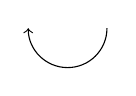
\begin{tikzpicture}[baseline=(A), scale=0.5]
			\coordinate (A) at (0, -0.5);
			\draw[<-] (0, 0) arc[radius=1, start angle=180, end angle=360];
		\end{tikzpicture} \; , \quad
		\mathrm{coev}_X := X \times
		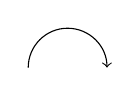
\begin{tikzpicture}[baseline=(A), scale=0.5]
			\coordinate (A) at (0, 0.2);
			\draw[->] (0, 0) arc[radius=1, start angle=180, end angle=0];
		\end{tikzpicture} \; .
	\end{gather*}
	\begin{itemize}
		\item Seperti dalam rujukan di atas, definisi $n\dcate{Cob}$ telah
		memuat bijeksi
		% segment-id: o014.li2.chapter9.duality-examples-a.q012
		\begin{align*}
			\Hom_{n\dcate{Cob}}(X, Y) & \xleftrightarrow{1:1} \Hom_{n\dcate{Cob}}\left( \emptyset, X^* \sqcup Y\right) \\
			& = \left\{ W: \text{berorientasi dengan batas, beserta data}\; \partial W \rightiso X^* \sqcup Y \right\} / \sim .
		\end{align*}
		\item Dual sebuah morfisme, yakni kobordisme, hanya membalik
		$\partial W\rightiso X^*\sqcup Y$ menjadi
		$\partial W\rightiso(Y^*)^*\sqcup X^*$.
		\item Jejak dan dimensi mengambil nilai dalam
		% segment-id: o014.li2.chapter9.duality-examples-a.q013
		\[ \End_{n\dcate{Cob}}(\emptyset)=
		\{\text{manifold kompak tanpa batas berdimensi }n\}/\sim . \]
		\item Menurut deskripsi $\mathrm{ev}_X$ dan $\mathrm{coev}_X$ di
		atas, mengambil jejak $f\in\End_{n\dcate{Cob}}(X)$ berarti merekatkan
		dua ujung $X$ pada kobordisme $f$. Karena morfisme identitas
		$\identity_X$ bersesuaian dengan kobordisme trivial
		$X\times[0,1]$, kita memperoleh
		% segment-id: o014.li2.chapter9.duality-examples-a.q014
		\[ \dim X = X \times
		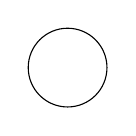
\begin{tikzpicture}[baseline=(O), scale=0.5]
			\coordinate (O) at (0, -0.25);
			\draw (0, 0) circle[radius=1];
		\end{tikzpicture} \; . \]
	\end{itemize}

	Untuk $n\dcate{Cob}$, berbagai diagram yang diperkenalkan dalam
	\S\ref{sec:monoidal-dual} memperoleh makna literal. Metode dan objek di
	sini memiliki hakikat geometris yang sama.
\end{example}
